\documentclass[]{article}
\usepackage{tikz}
\usepackage{graphics}
\usepackage{graphicx}
\usepackage{pst-node,pst-plot}
\usepackage{svg}

%opening
\title{Practical implementation for fair exchange of two pieces of information using a single Bitcoin transaction involving punishment for non-cooperating party}
\author{Shahpour Moavenat}
\begin{document}

\maketitle

\begin{abstract}
There are some problems in which it is required to exchange two pieces of information between parties who do not trust each other, two of these problems are mentioned in the next section. This problem has been vastly studied, for example in \cite{ray2002} and \cite{asokan99}. In this article a method is presented so that by building and publishing a bitcoin transaction, each party should either reveal the agreed upon piece of information or if after some designated time passed, pay an agreed upon sum of Bitcoin to the other party.

\textbf{Related work:} A similar high level study is available including some suggestions to change Bitcoin protocol in \cite{andrychowicz}.
\end{abstract}

\section{Introduction}
Two samples of the problems of interest are: a- Assuming two parties have sent two different assets to each other through a configuration of lightning network \cite{lightning} and the assets have arrived locked by a pre-image (R). If now parties exchange the pre-images, actually they can exchange their assets. b- Assume two parties want to exchange their signatures for example (RSA signatures on a document), the desired final state is that either each party should have the others signatures or neither should have the other's one (zkSNARK to make sure what is provided is actually the signature). When strong fairness is required (which roughly means at end of exchange either both parties have the required information or no party has any additional information about the other party item) this problems is proved not to be solvable in peer-to-peer without a trusted third party \cite{impossible}.

\section{Bitcoin transaction with penalty}
Using Bitcoin network, we can ask each party to put a collateral in Bitcoin transaction that will be returned to him/her when (s)he contributes the secret publicly, otherwise after some timeout the collateral will be spendable by the other party. By using this method each party is forced to release the secret or pay a penalty, if (s)he does not do so.

The transaction should be of segregated witness \cite{segwit} type, so its transaction id could be known without signatures and monitored on blockchain, when a party who signs the transaction the second, if did not broadcast the transaction (which may have lower probability, since before this signature exchange phase, both parties have followed some other procedures and somehow showed their intentions for exchange; although more analysis may be required here), the transaction could be monitored for further actions.

So the built transaction will have two inputs and two outputs, two inputs are the collaterals each party puts in to the contract so that it could be punished if the release of desired information is not done in the desired time frame.

\subsection{Transaction details}

The desired transaction will have 2 inputs, and two outputs, as in Figure \ref{fig:transaction}.

\begin{figure}[h!]
	\centering
	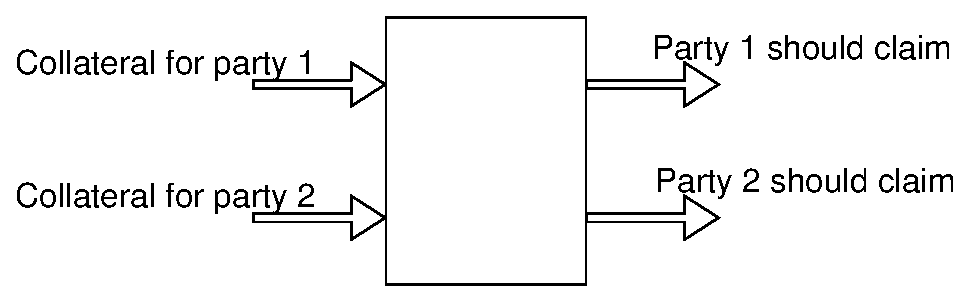
\includegraphics[width=1\textwidth]{images/transaction.eps}
	\caption{Segwit transaction	to be signed and posted to blockchain}
	\label{fig:transaction}
\end{figure}

Input amounts are what each party needs to put into transaction (contract) as collateral, that if the corresponding output was not claimed, will become available to the other party after sometime as a mechanism of punishment for not following the protocol. If the output is claimed, this will release the information required for the exchange.

Output script will generally be like following (Actual details will depend on the hash type):

\begin{verbatim}
OP_SHA256
<Y> OP_EQUAL
OP_IF
<Self Pubkey>
OP_ELSE
<block_height+number of blocks in the required timeout period> OP_CHECKLOCKTIMEVERIFY OP_DROP
<Other party Pubkey>
OP_ENDIF
OP_CHECKSIG
\end{verbatim}

The above output could be claimed by the party putting collateral, if it releases the pre-image of the hash. Otherwise after some designated time, the other party could claim the collateral as punishment for not releasing the pre-image. So if every party is interested in claiming its collateral (which normally should be case), the result would be release of pre-images to blockchain which means every party would become aware of the other party's pre-image and exchange of pre-images has happened.

\section{Conclusion}
a- zkSNARK to make sure exchanged information is what they should be as described.
b- Problem of second signing party not broadcasting the transaction


\begin{thebibliography}{9}
	\bibitem{ray2002}
	Indrajit Ray, Indrakshi Ray, 
	\textit{Fair Exchange in E-commerce},
	ACM SIGecom Exchanges, Volume 3 Issue 2, Spring, 2002,
	pp 9-17. 
	
	\bibitem{asokan99}
	    N. Asokan,Victor Shoup,Michael Waidner,
	    \textit{Optimistic fair exchange of digital signatures},
	    revised and extended version of Eurocrypt 99 Abstract and of IBM research report RZ 2973, 1999. Available from http://www.shoup.net/papers/fex.pdf
		
	\bibitem{maxwell2016}
	Gregory Maxwell,
	\textit{The first successful Zero-Knowledge Contingent Payment}, 2016.
	Available from https://bitcoincore.org/en/2016/02/26/zero-knowledge-contingent-payments-announcement/
	
	\bibitem{andrychowicz}
	Marcin Andrychowicz, Stefan Dziembowski, Daniel Malinowski, Lukasz Mazurek,
	\textit{Fair Two-Party Computations via Bitcoin Deposits}, Financial Cryptography and Data Security: FC 2014 Workshops, BITCOIN and WAHC 2014, Christ Church, Barbados, March 7, 2014, Revised Selected Papers, pp 105-121.
	
	\bibitem{segwit}
	Eric Lombrozo, Johnson Lau, Pieter Wuille,
	\textit{Segregated Witness Bitcoin Improvement Proposal},
	Available from https://github.com/bitcoin/bips/blob/master/bip-0141.mediawiki
	
	\bibitem{impossible}
	H. Pagnia, F. C. Gärtner, 
	\textit{On the impossibility of fair exchange without a trusted
	third party}, Technical report, 1999.

	\bibitem{lightning}
	Joseph Poon, Thaddeus Dryja,
	\textit{The Bitcoin Lightning Network: Scalable Off-Chain Instant Payments}, DRAFT Version 0.5.9.2, 2016.
	    
\end{thebibliography}
\end{document}
